\section{Конструкторский раздел}
\setcounter{figure}{0}
\setcounter{table}{0}

\subsection{Определение переменного темпа}

На рисунках \ref{img:tempo_0} -- \ref{img:tempo_3} приведены IDEF0-диаграммы для метода определения переменного темпа музыки.

\begin{figure}[h]
	\centering
	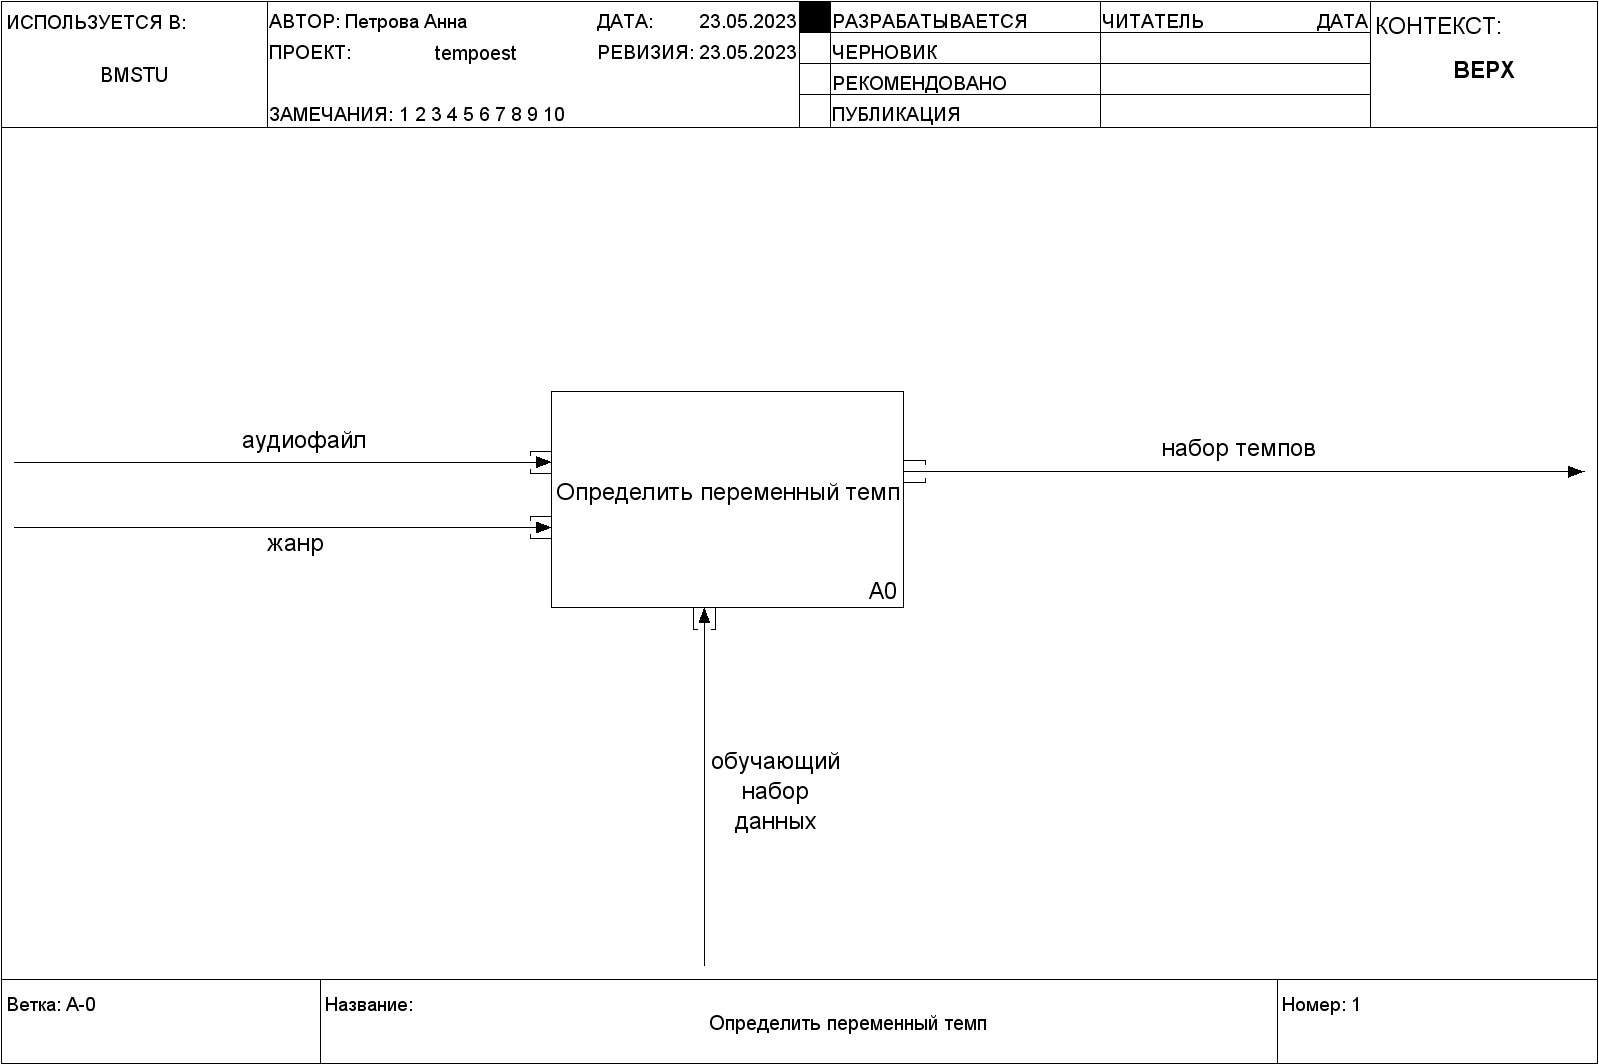
\includegraphics[scale=0.25]{inc/img/tempo_idef/01_A-0.png}
	\caption{IDEF0 нулевого уровня}
	\label{img:tempo_0}
\end{figure}

Для адаптации используемого метода к определению переменного темпа музыки анализируемый аудиофайл разделяется на равные фрагменты. Опытным путем было выявлено, что оптимальной длиной фрагментов является 5 секунд. Если взять более короткие фрагменты, то методу начинает не хватать данных для определения темпа из-за слишком маленькой длины аудио. При этом если разделять на более крупные фрагменты, то увеличивается риск пропуска изменений темпа.

\begin{figure}[h]
	\centering
	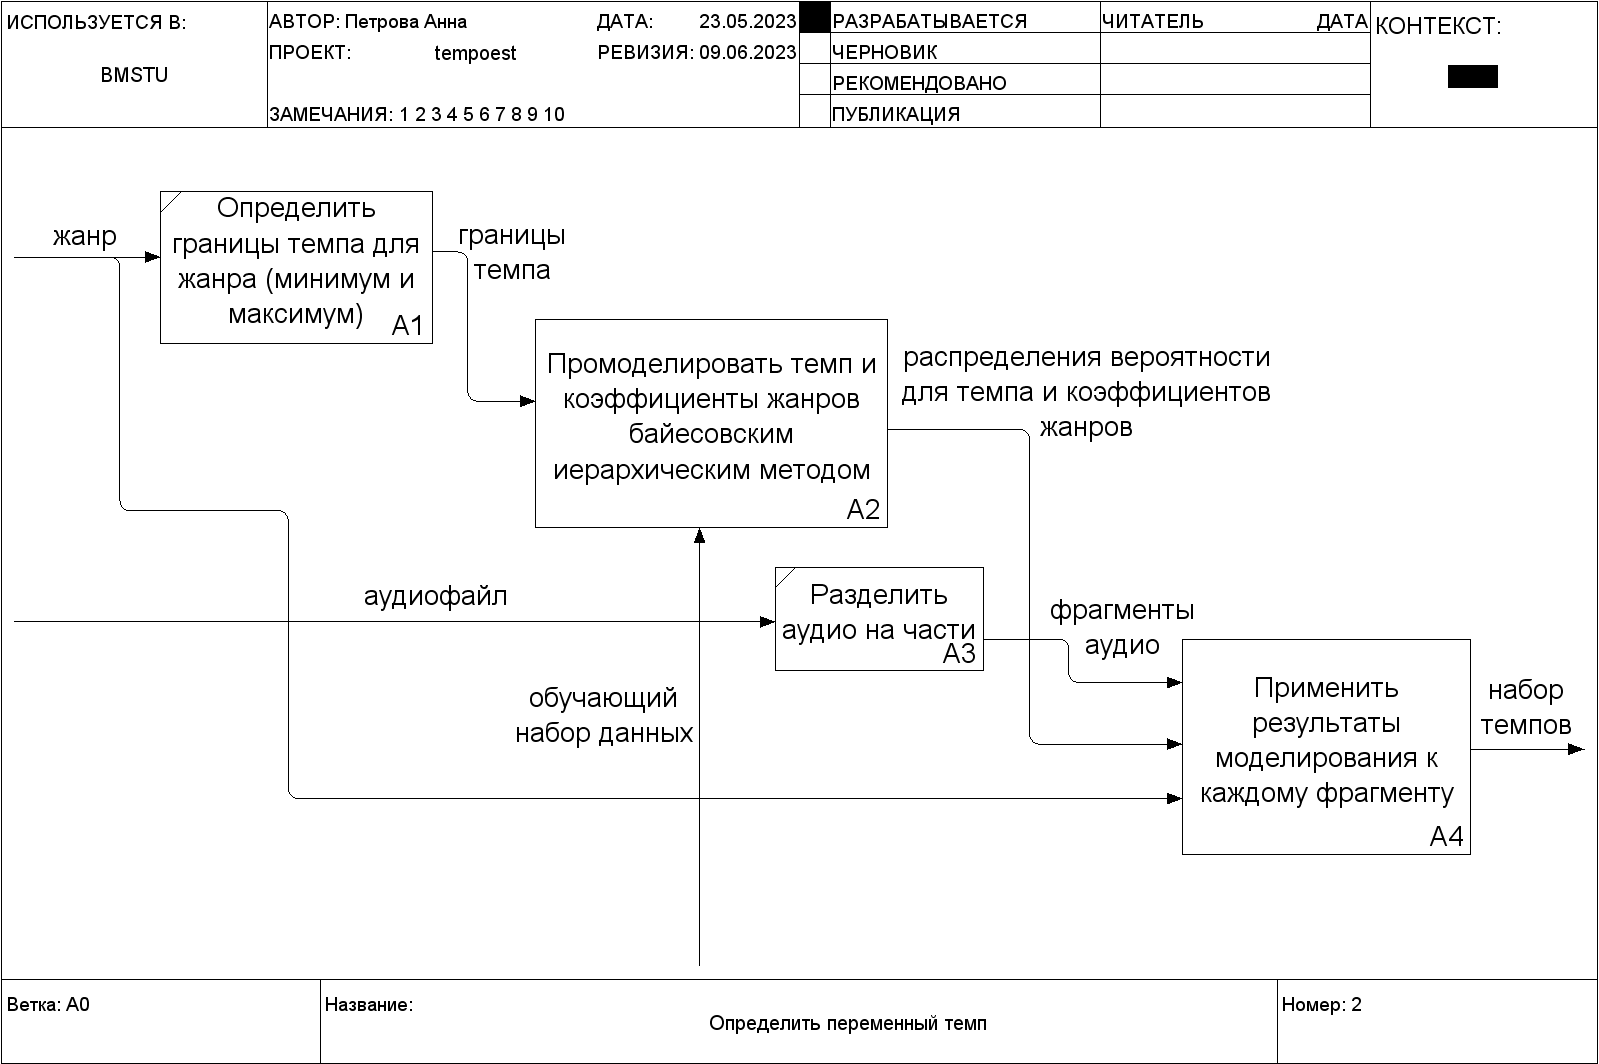
\includegraphics[scale=0.25]{inc/img/tempo_idef/02_A0.png}
	\caption{Определение переменного темпа}
	\label{img:tempo_1}
\end{figure}

При реализации байесовской иерархической модели в качестве априорного распределения темпа анализируемой музыки было выбрано равномерное распределение с границами от минимального возможного темпа до максимального. Границы темпа выбираются на основе указанного жанра музыки. Такое распределение было выбрано, так как на данном этапе, за неимением каких-либо других характеристик указанного аудиофайла, предполагается, что все темпы для него в заданных пределах равновероятны.

Коэффициенты жанров необходимы для корректировки получаемой оценки темпа в зависимости от жанра музыки. Если коэффициент отрицательный, то темп должен быть уменьшен, если положительный -- увеличен. В качестве априорного распределения коэффициентов для всех жанров было выбрано нормальное распределение с математическим ожиданием, равным 0, и дисперсией, равной 1. Такой выбор связан с тем, что чаще всего разница между темпами в зависимости от жанра не слишком большая. Это означает, что корректирующие коэффициенты с большей вероятностью находятся в <<районе>> нуля. При этом 0 является <<нейтральным>> коэффициентом, т.~е. не влияет на полученную оценку темпа.

На основе информации из датасета было выявлено, что распределение темпов различной музыки близко к нормальному (рис.~\ref{img:bpm_distribution}).

\begin{figure}[h]
	\centering
	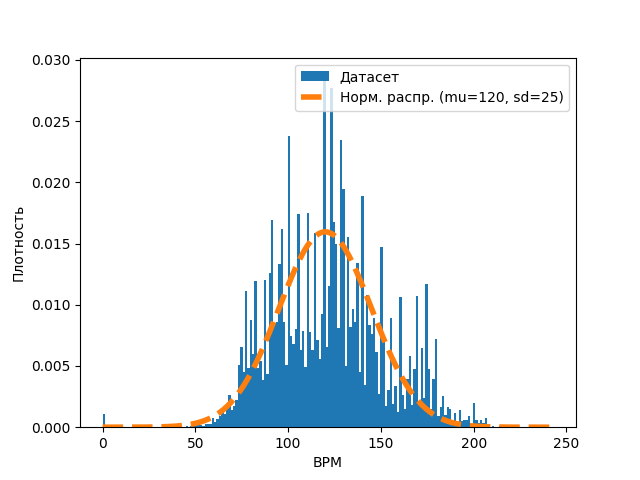
\includegraphics[scale=0.7]{../graphs/bpm_distribution.png}
	\caption{Распределение темпов музыки из датасета}
	\label{img:bpm_distribution}
\end{figure}

Поэтому в качестве распределения функции правдоподобия темпа было выбрано нормальное распределение. Математическое ожидание для каждого жанра для этого распределения рассчитывается на основе мат. ожидания и дисперсии априорного распределения темпа и априорных распределений коэффициентов жанров по формуле:
\begin{equation}
	\mu = \mu_{\text{prior}} + \text{coef} * \sigma_{\text{prior}},
\end{equation}

где $\mu_{\text{prior}}$ -- мат. ожидание априорного распределения темпа, $\sigma_{\text{prior}}$ -- дисперсия априорного распределения темпа, coef -- априорный коэффициент текущего жанра.

В качестве дисперсии при этом используется дисперсия априорного распределения темпа.

\begin{figure}[h]
	\centering
	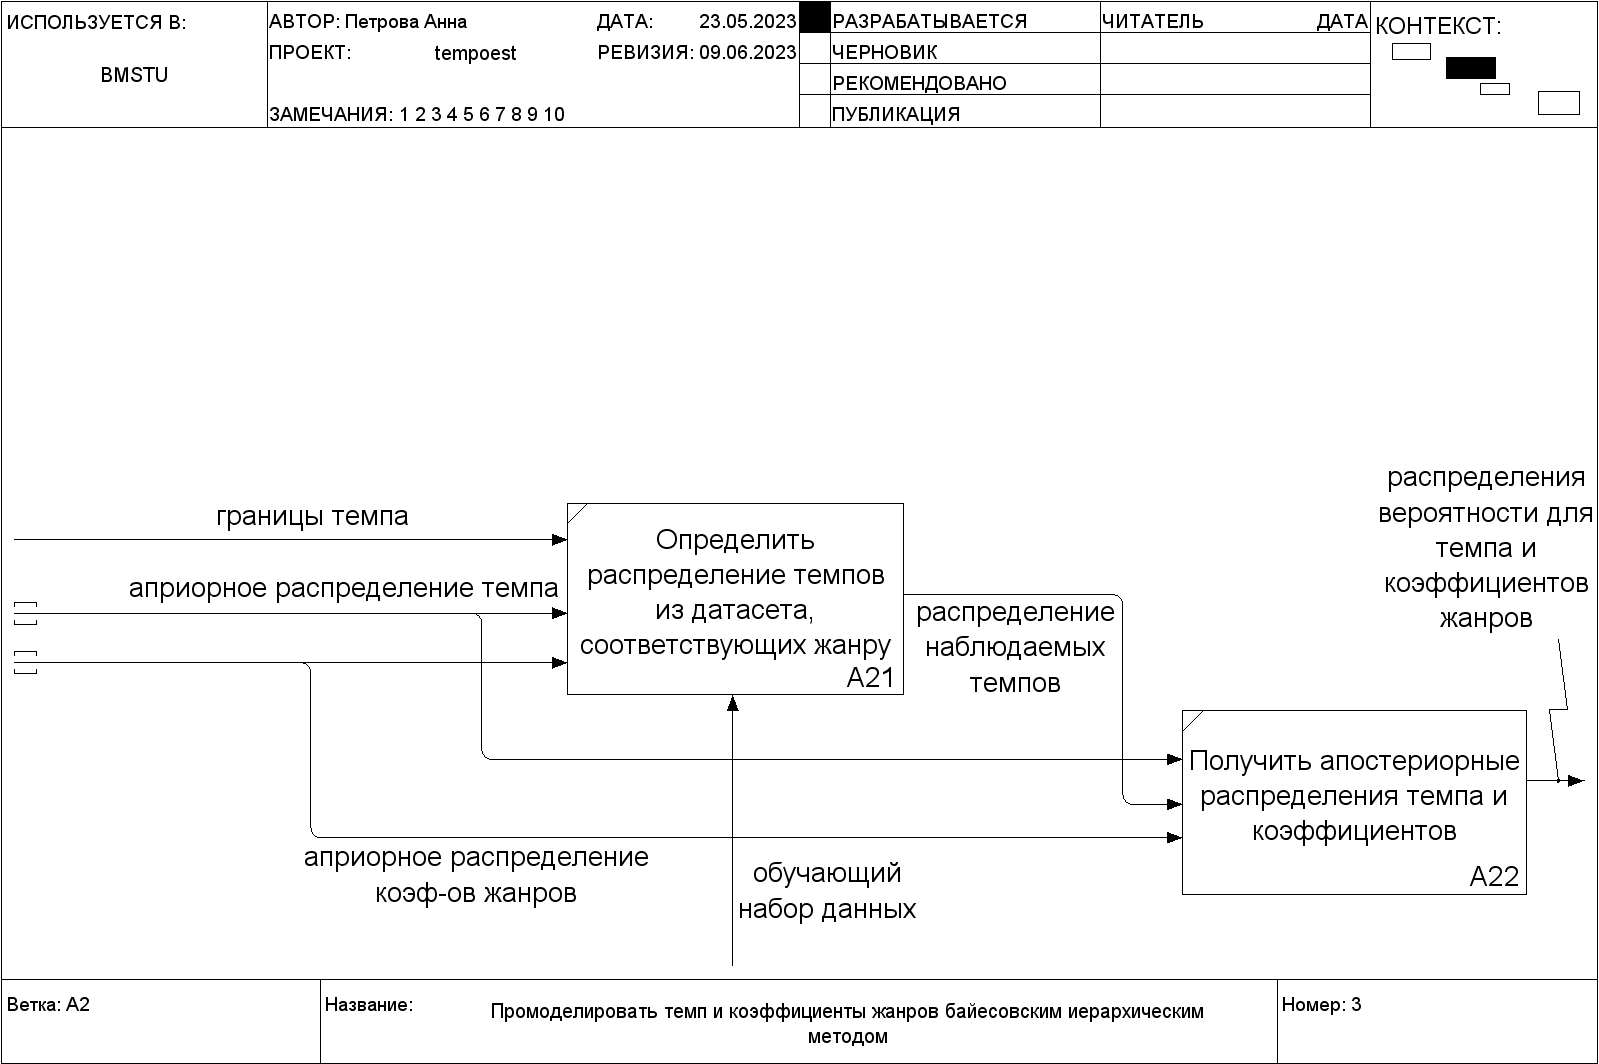
\includegraphics[scale=0.25]{inc/img/tempo_idef/03_A2.png}
	\caption{Байесовское моделирование}
	\label{img:tempo_2}
\end{figure}

Важно заметить, что в самой байесовской модели не используется анализируемый аудиофайл. В результате подсчета модели получаются апостериорные распределения темпа для заданного жанра в заданных границах и коэффициентов жанров.

После моделирования для каждого фрагмента аудиофайла рассчитывается примерный диапазон возможных темпов. Для этого сначала определяются так называемые <<силы нажатия>> на ноты, то есть амплитуды сигнала во временной области, после чего определяется приблизительное значение темпа на основе корреляции этих амплитуд. Далее относительно найденного темпа делается разброс значений в определенном интервале. Этот диапазон <<накладывается>> на полученное байесовским моделированием распределение темпа, и получается наиболее вероятный темп (максимум плотности распределения) в данном диапазоне (tempo) (рис.~\ref{img:res_tempo}).

После этого среди апостериорных распределений коэффициентов жанров находится распределение для указанного жанра. В этом распределении ищется наиболее вероятный коэффициент (coef). После чего применяется формула:
\begin{equation}
	\text{result} = \text{tempo} + \text{coef} * \sigma_{\text{prior}}.
\end{equation}

\begin{figure}[h]
	\centering
	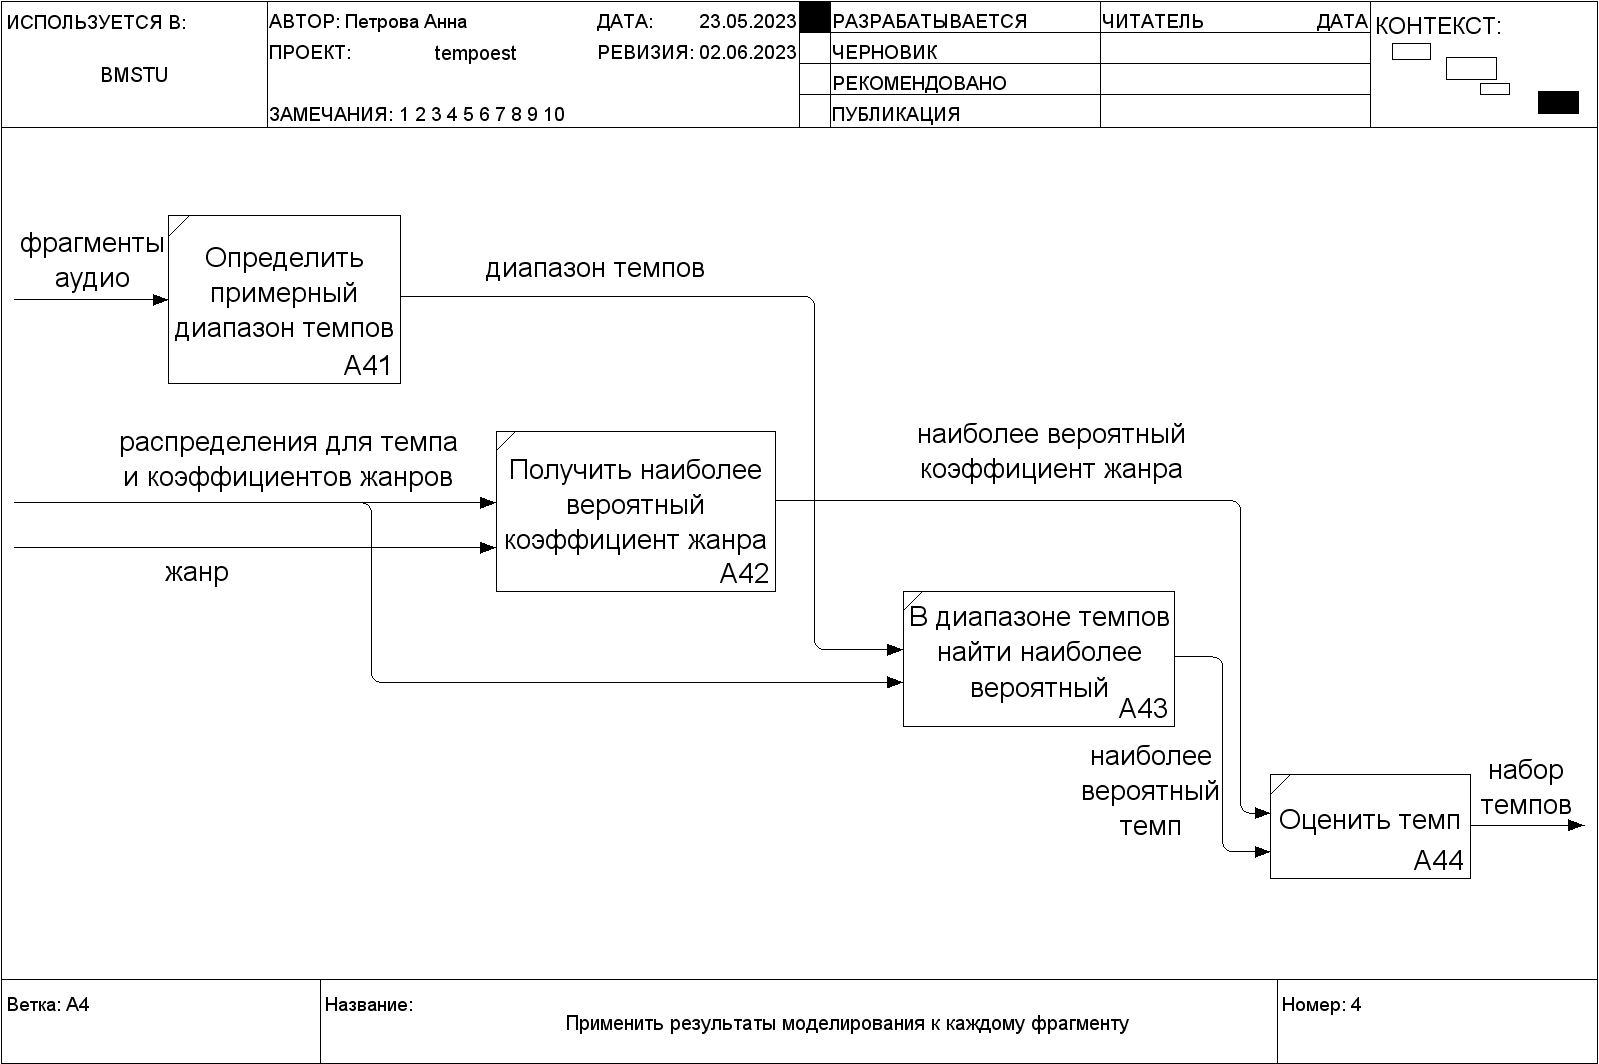
\includegraphics[scale=0.25]{inc/img/tempo_idef/04_A4.png}
	\caption{Применение результатов к фрагментам аудио}
	\label{img:tempo_3}
\end{figure}

\begin{figure}[h]
	\centering
	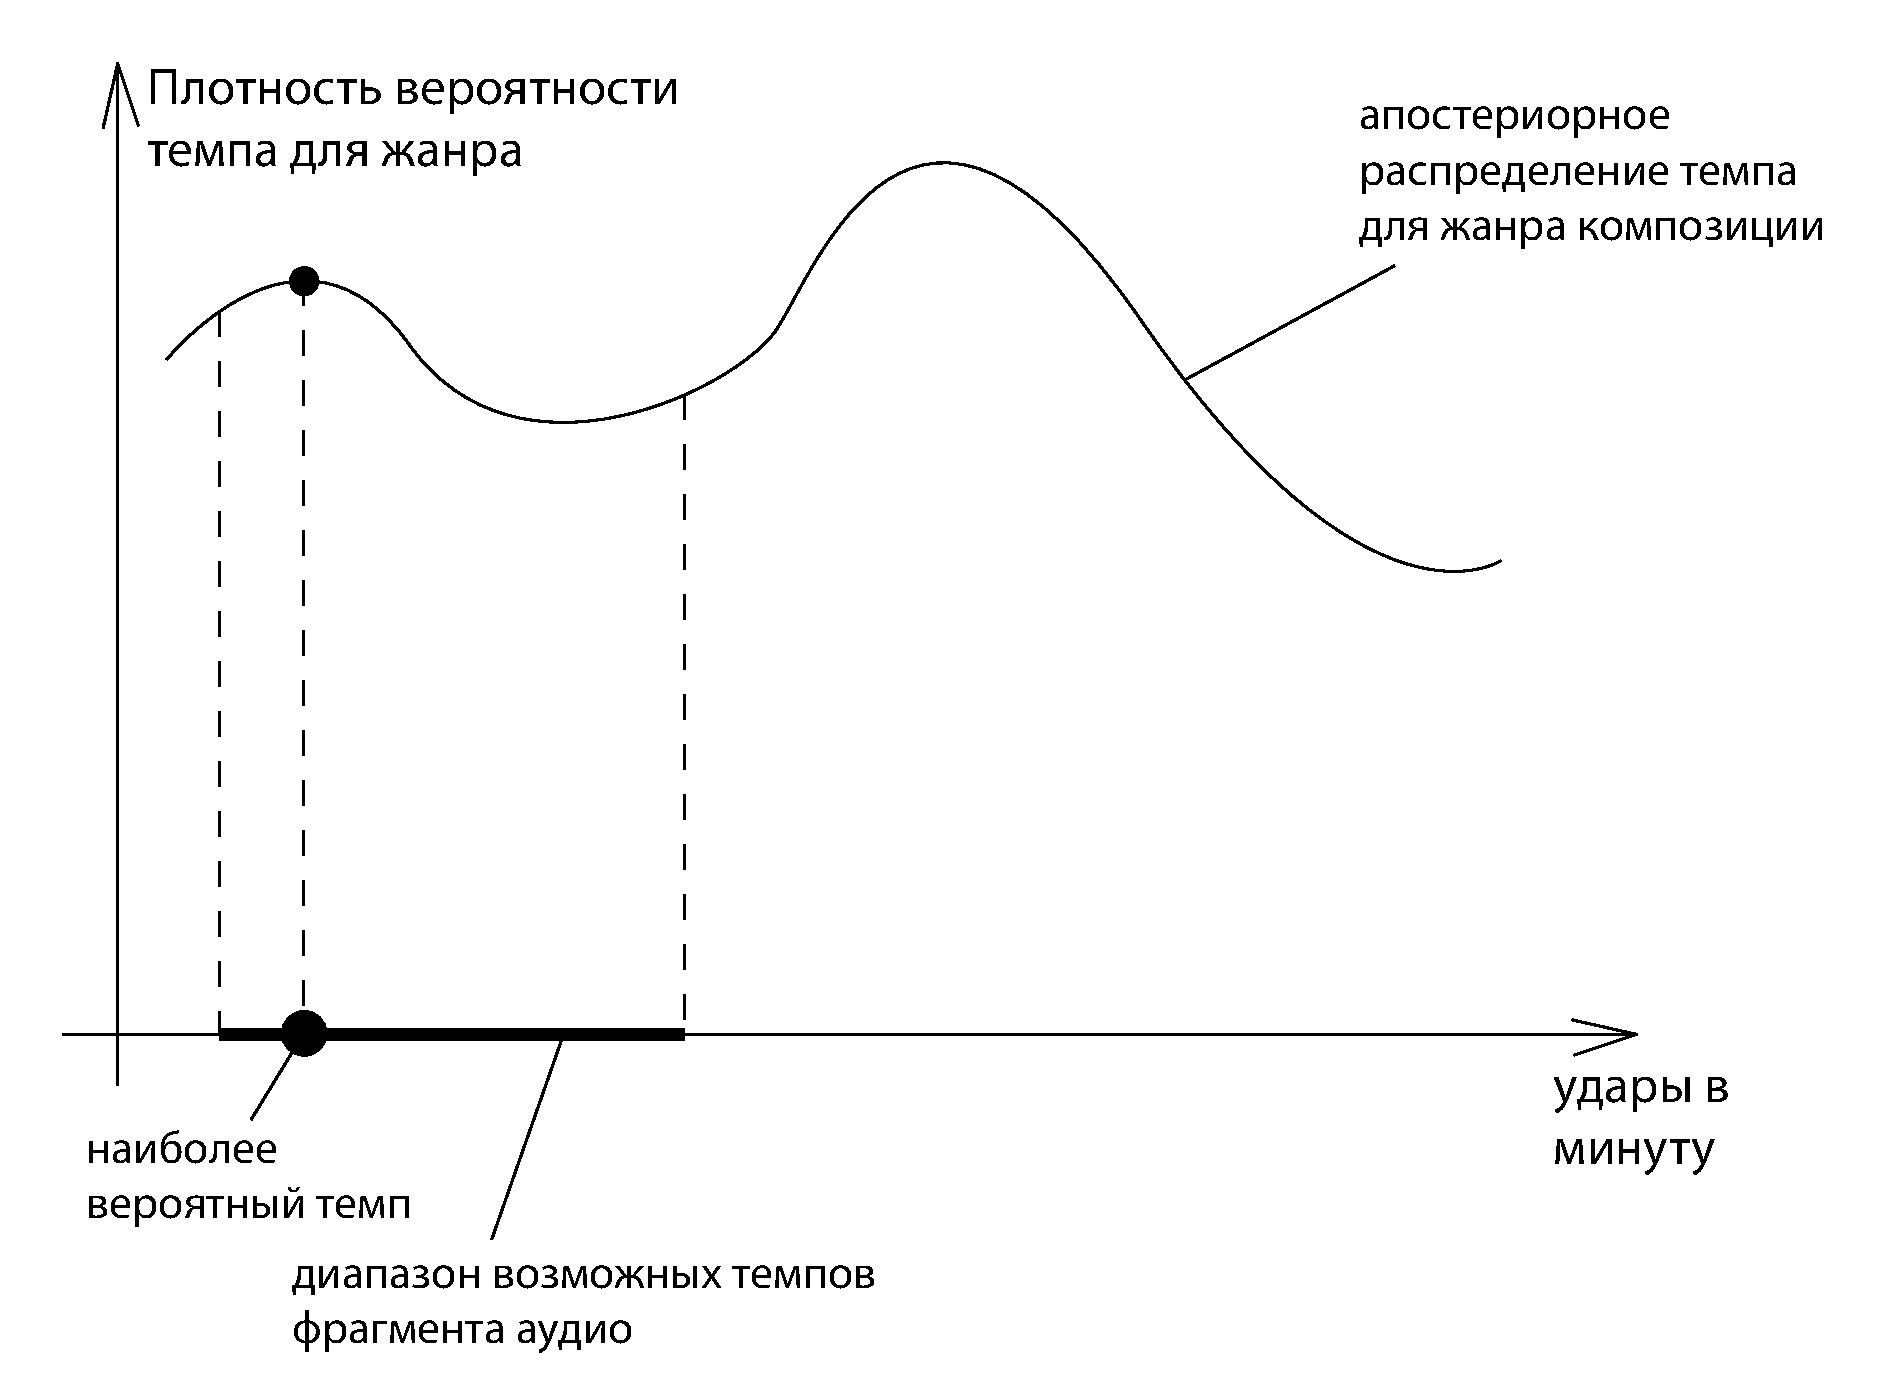
\includegraphics[scale=0.5]{svg/res_tempo.pdf}
	\caption{Нахождение наиболее вероятного темпа}
	\label{img:res_tempo}
\end{figure}

\clearpage

\subsection{Определение переменного ритма}

На рисунках \ref{img:rhythm_0} -- \ref{img:rhythm_3} приведены IDEF0-диаграммы для алгоритма определения переменного ритма (тактового размера) музыки.

\begin{figure}[h]
	\centering
	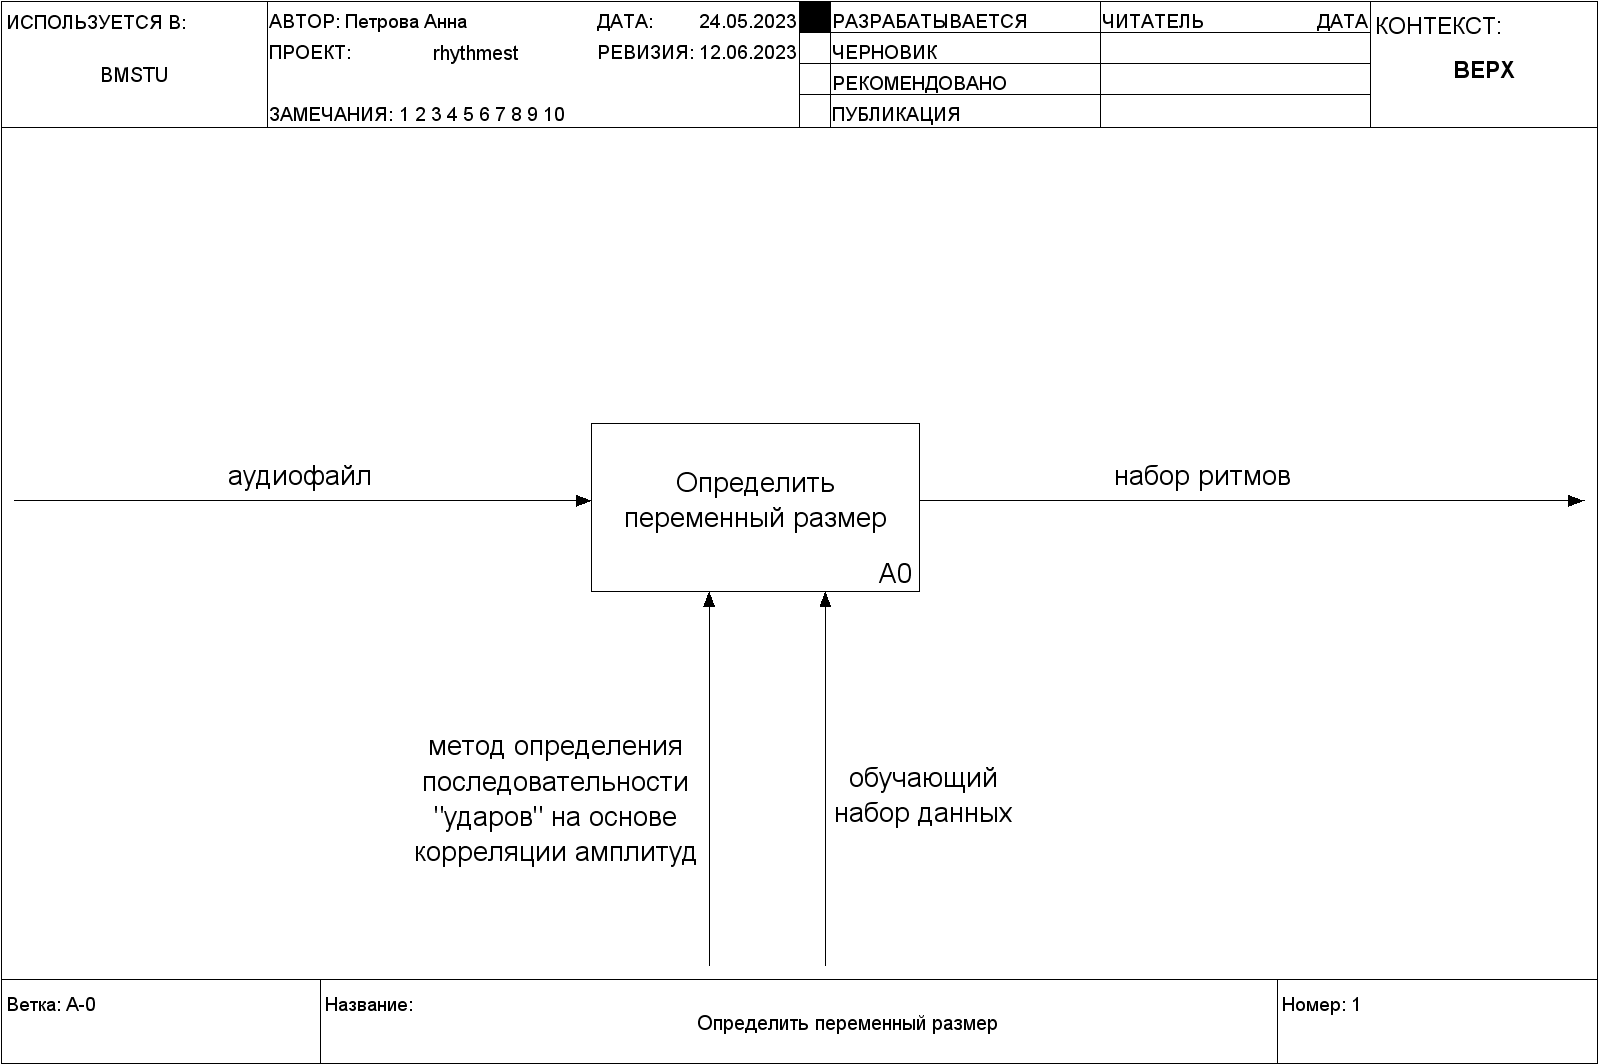
\includegraphics[scale=0.25]{inc/img/rhythm_idef/01_A-0.png}
	\caption{IDEF0 нулевого уровня}
	\label{img:rhythm_0}
\end{figure}

По аналогии с определением темпа в качестве априорного распределения тактового размера в байесовской модели выбрано равномерное распределение, так как на данном этапе, за неимением каких-либо других характеристик указанного аудиофайла, предполагается, что все размеры для него в заданных пределах равновероятны.

В качестве распределения функции правдоподобия размера выбрано нормальное распределение (поскольку распределение размеров в датасете также близко к нормальному) с математическим ожиданием, равным математическому ожиданию априорного, и дисперсией, также равной априорной.

\begin{figure}[h]
	\centering
	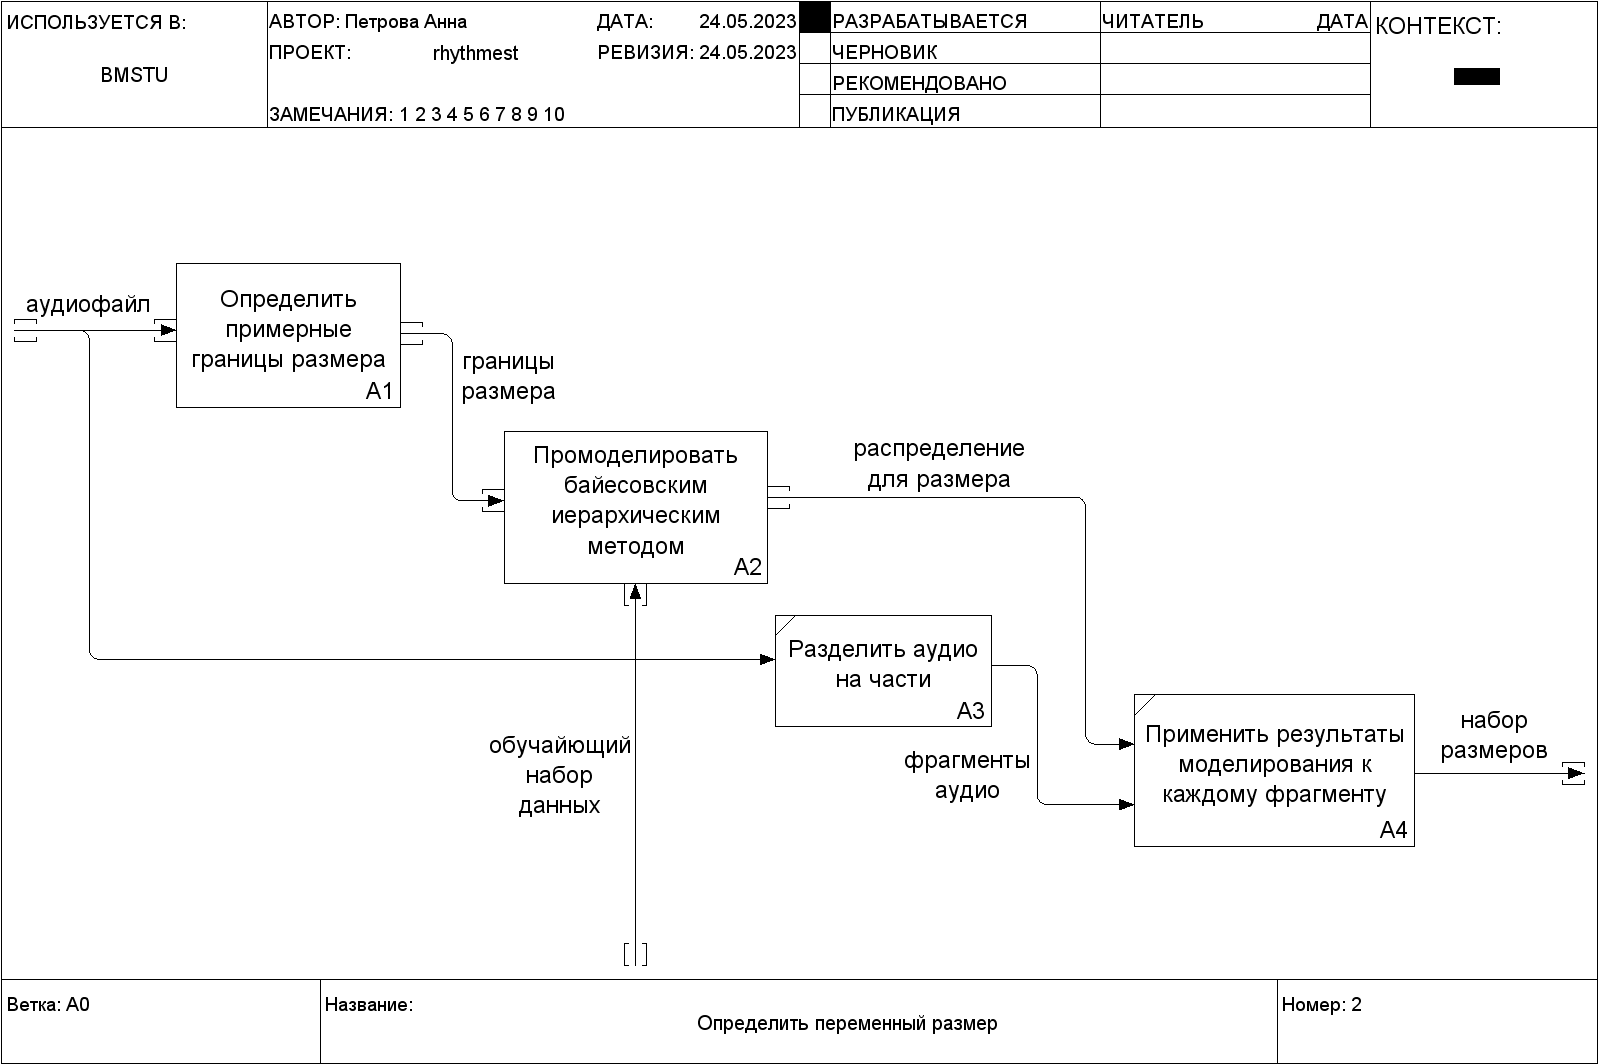
\includegraphics[scale=0.25]{inc/img/rhythm_idef/02_A0.png}
	\caption{Определение переменного ритма}
	\label{img:rhythm_1}
\end{figure}

\begin{figure}[h]
	\centering
	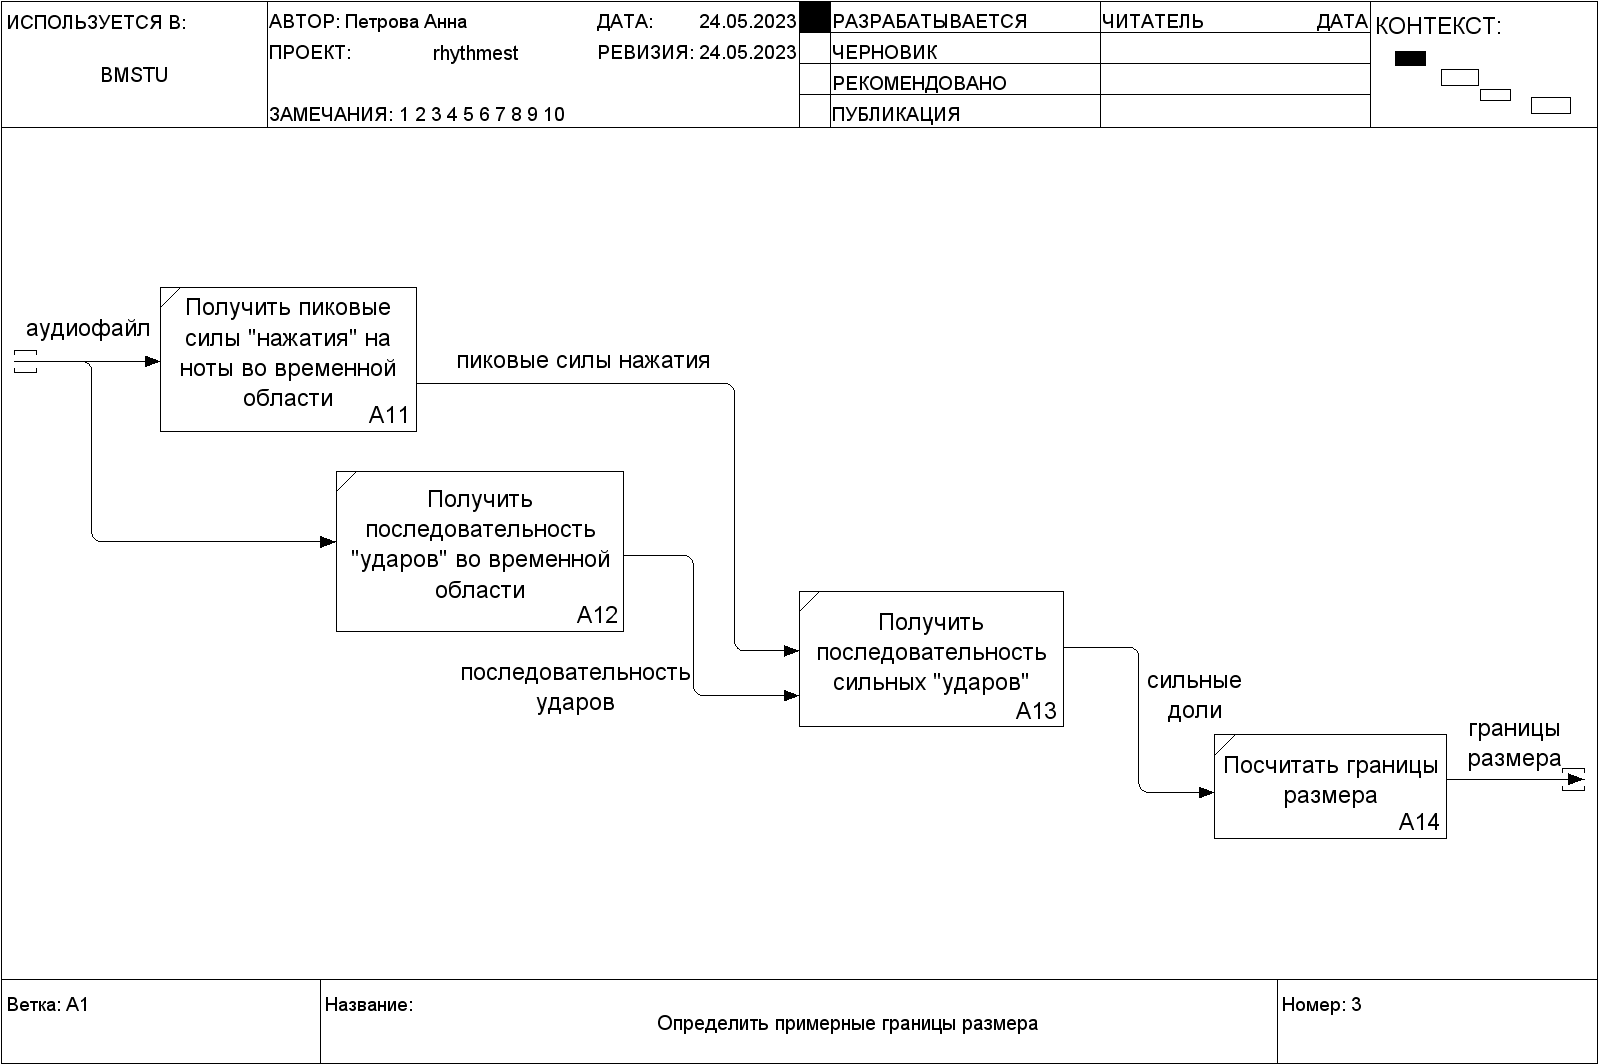
\includegraphics[scale=0.25]{inc/img/rhythm_idef/03_A1.png}
	\caption{Определение границ размера}
	\label{img:rhythm_2}
\end{figure}

\newpage

Для задания априорного распределения необходимо определить границы размера. Для этого во всем аудиофайле сначала находятся последовательности амплитуд и <<ударов>> во временной области. Последовательность <<ударов>> определяется на основе оценки темпа. В найденной последовательности амплитуд находятся пики (точки максимума). После чего пики амплитуд <<накладываются>> на последовательность <<ударов>> и получается последовательность сильных <<ударов>> (долей) (т.~е. предположительные начала тактов). Количество <<ударов>> между сильными долями и есть тактовый размер. Таким образом определяются примерные границы размеров рассматриваемого аудиофайла.

Остальное происходит аналогично определению темпа. Считается байесовская модель для оценки апостериорной вероятности размера. Далее аудиофайл разделяется на фрагменты по 5 секунд, для каждого фрагмента рассчитывается диапазон размеров по принципу, описанному выше. После чего полученное в результате моделирования апостериорное распределение размеров применяется к данному диапазону, и ищется максимум функции плотности, т.~е. наиболее вероятный тактовый размер фрагмента.

\begin{figure}[h]
	\centering
	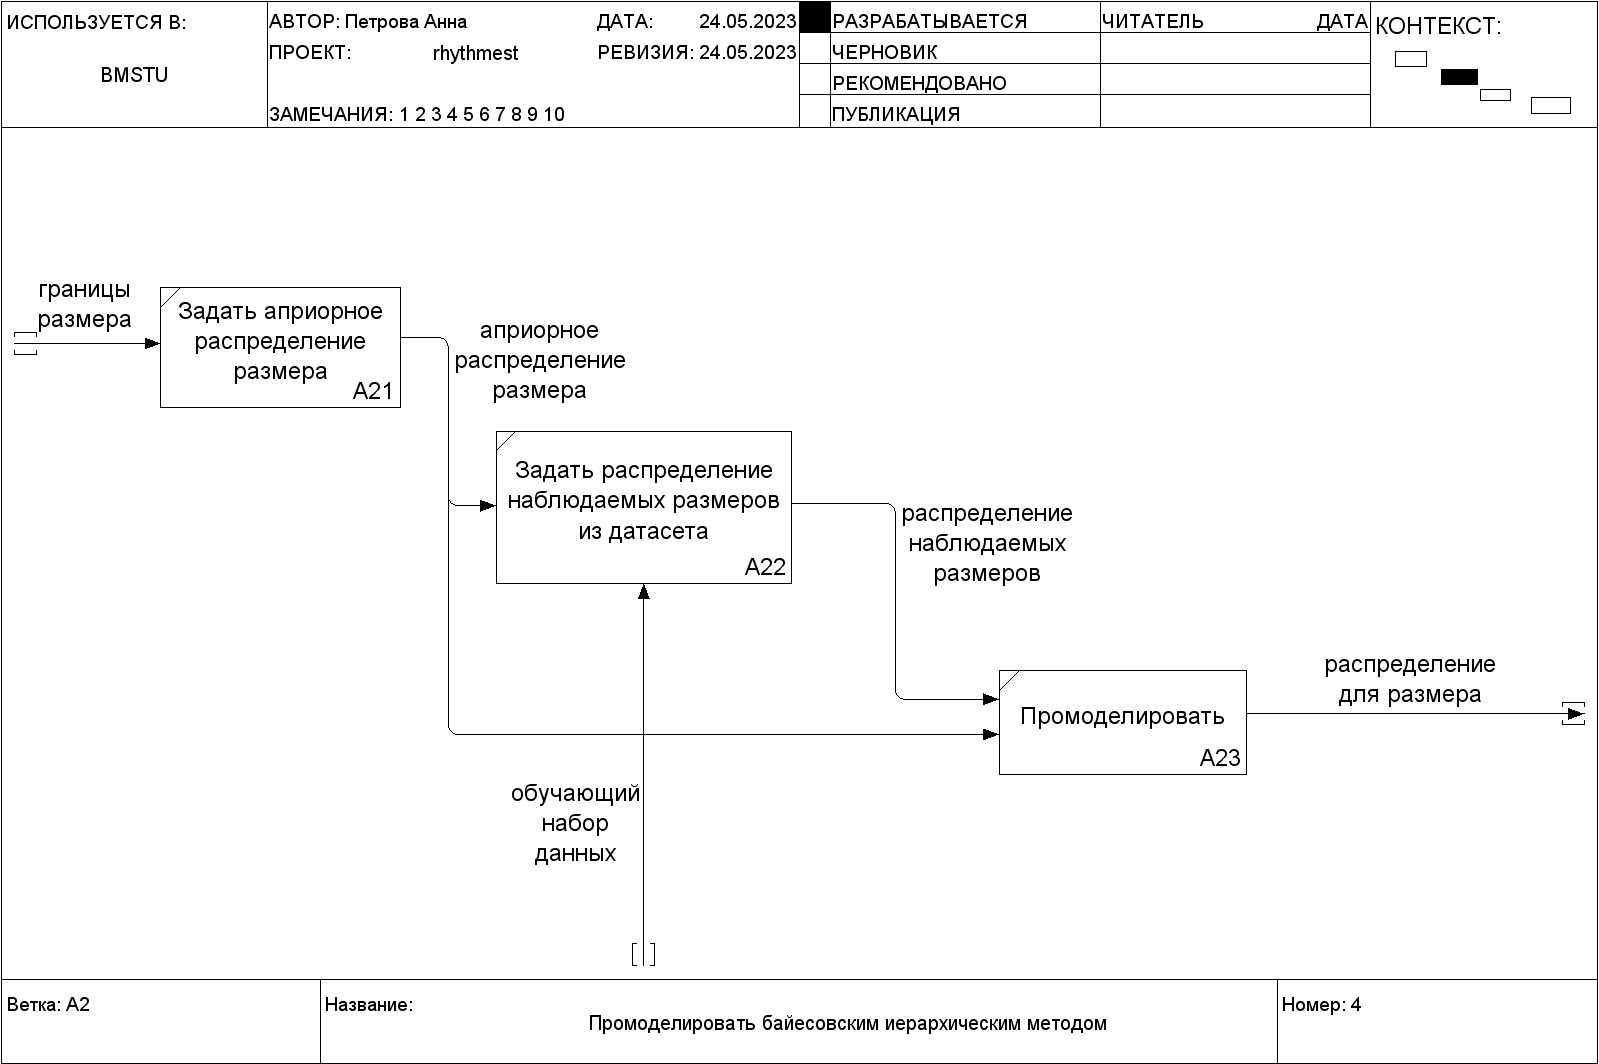
\includegraphics[scale=0.25]{inc/img/rhythm_idef/04_A2.png}
	\caption{Байесовское моделирование}
	\label{img:rhythm_3}
\end{figure}

\clearpage

\subsection{Структуры данных}

Результаты работы программы будут представлены в виде словарей, где в качестве ключей -- время от начала аудиофайла в секундах, а в качестве значений -- темпы или тактовые размеры соответственно.

Все распределения, значения из датасета, последовательности <<ударов>> и пики амплитуды будут представлены в виде списков. Списки <<ударов>> и пиков амплитуды представляют собой последовательность секунд от начала аудиозаписи, в которые происходят <<удары>> или пики амплитуды соответственно.

\subsection{Структура ПО}

На рисунке \ref{img:sw_structure} показана структура приложения, из которой видно, как происходит взаимодействие компонентов.

\begin{figure}[h]
	\centering
	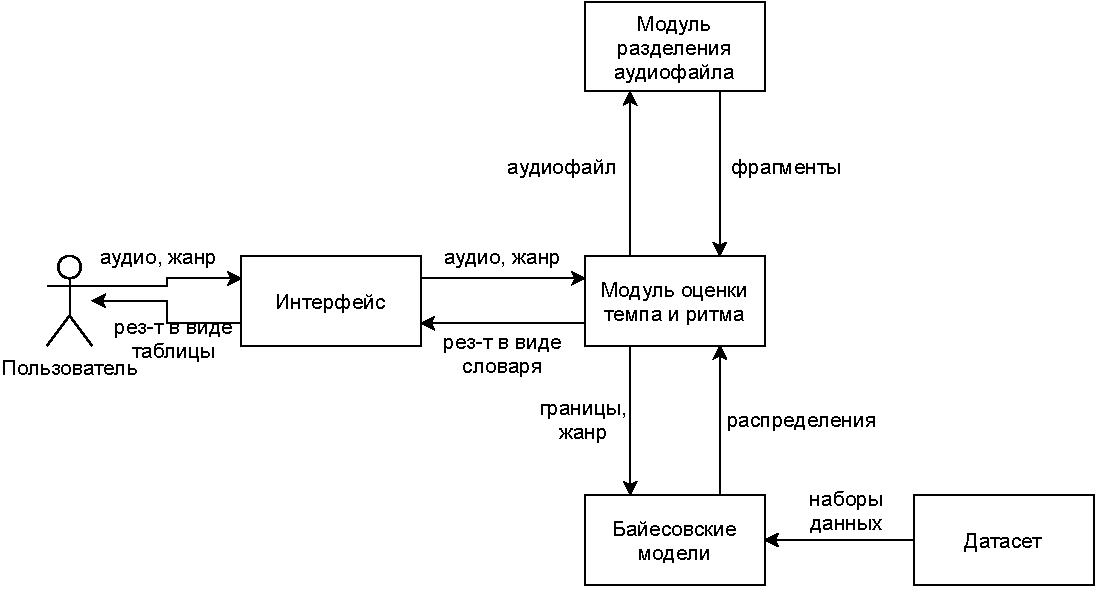
\includegraphics[scale=0.9]{svg/sw_structure.pdf}
	\caption{Структура приложения}
	\label{img:sw_structure}
\end{figure}

Модуль оценки темпа и ритма применяет результаты байесовского моделирования к фрагментам заданного аудиофайла.

\newpage

\subsection*{Выводы}

На основе теоретических данных, полученных в аналитическом разделе, был разработан метод определения переменного темпа и ритма музыки. Также были приведены IDEF0-диаграммы, схема структуры приложения и описаны основные структуры данных.

